\documentclass{article}\usepackage[]{graphicx}\usepackage[]{color}
%% maxwidth is the original width if it is less than linewidth
%% otherwise use linewidth (to make sure the graphics do not exceed the margin)
\makeatletter
\def\maxwidth{ %
  \ifdim\Gin@nat@width>\linewidth
    \linewidth
  \else
    \Gin@nat@width
  \fi
}
\makeatother

\definecolor{fgcolor}{rgb}{0.345, 0.345, 0.345}
\newcommand{\hlnum}[1]{\textcolor[rgb]{0.686,0.059,0.569}{#1}}%
\newcommand{\hlstr}[1]{\textcolor[rgb]{0.192,0.494,0.8}{#1}}%
\newcommand{\hlcom}[1]{\textcolor[rgb]{0.678,0.584,0.686}{\textit{#1}}}%
\newcommand{\hlopt}[1]{\textcolor[rgb]{0,0,0}{#1}}%
\newcommand{\hlstd}[1]{\textcolor[rgb]{0.345,0.345,0.345}{#1}}%
\newcommand{\hlkwa}[1]{\textcolor[rgb]{0.161,0.373,0.58}{\textbf{#1}}}%
\newcommand{\hlkwb}[1]{\textcolor[rgb]{0.69,0.353,0.396}{#1}}%
\newcommand{\hlkwc}[1]{\textcolor[rgb]{0.333,0.667,0.333}{#1}}%
\newcommand{\hlkwd}[1]{\textcolor[rgb]{0.737,0.353,0.396}{\textbf{#1}}}%

\usepackage{framed}
\makeatletter
\newenvironment{kframe}{%
 \def\at@end@of@kframe{}%
 \ifinner\ifhmode%
  \def\at@end@of@kframe{\end{minipage}}%
  \begin{minipage}{\columnwidth}%
 \fi\fi%
 \def\FrameCommand##1{\hskip\@totalleftmargin \hskip-\fboxsep
 \colorbox{shadecolor}{##1}\hskip-\fboxsep
     % There is no \\@totalrightmargin, so:
     \hskip-\linewidth \hskip-\@totalleftmargin \hskip\columnwidth}%
 \MakeFramed {\advance\hsize-\width
   \@totalleftmargin\z@ \linewidth\hsize
   \@setminipage}}%
 {\par\unskip\endMakeFramed%
 \at@end@of@kframe}
\makeatother

\definecolor{shadecolor}{rgb}{.97, .97, .97}
\definecolor{messagecolor}{rgb}{0, 0, 0}
\definecolor{warningcolor}{rgb}{1, 0, 1}
\definecolor{errorcolor}{rgb}{1, 0, 0}
\newenvironment{knitrout}{}{} % an empty environment to be redefined in TeX

\usepackage{alltt}
\usepackage{url}
\usepackage{amsmath}
\usepackage{amsfonts}
\usepackage[backend=bibtex, natbib=true]{biblatex}
\addbibresource{references.bib}


\usepackage[margin=1in]{geometry}
\setlength{\parindent}{0in}

\title{Accessing Data with the Census Bureau API}
\author{Alex Shum}
\IfFileExists{upquote.sty}{\usepackage{upquote}}{}
\begin{document}
\maketitle

\section{Abstract}
Placeholder.

\section{Introduction}
The United States Census Bureau has been conducting a decennial census since 1790.  Originally this census was a simply to count the population across the country.  More recently the decennial census includes a short-form asking for name, sex, age, and a few other demographic variables.  About one in six households also received a long-form that contained additional socioeconomic questions.  After the 2000 decennial census many of the long-form questions were collected as part of a new survey: the American Community Survey (ACS).  \\
\\
The ACS is an ongoing yearly survey that collects additional demographic variables including but not limited to age, sex, race, income and education.  Unlike the decennial census, the American Community Survey is distributed based on a random selection of addresses every year.  Although the ACS is only sent to a sample of all US households, this data is meant to provide more up to date information than the Census Bureau's decennial census.  Both the decennial census and the American Community Survey are required to be completed by law; however it should be noted that the Census Bureau has not opted to prosecute anyone for failure to complete the decennial census or the ACS.  Despite the lack of enforcement, the ACS still reports a response rate of 97$\%$.\\ %http://www.politifact.com/texas/statements/2014/jan/09/us-census-bureau/americans-must-answer-us-census-bureau-survey-law-/
\\
Both the decennial survey and the ACS data are used in part by federal, state and local agencies to allocate state funding and for policy decisions.  The Census Bureau has also released some of this data for public use.  Many of the data sets are available directly in a compressed format from the Census Bureau's FTP site: \url{http://ftp2.census.gov/}.  Since 2012, the Census Bureau has also included an online developer's API in order to improve accessibility of the ACS and decennial census datasets.  The Census Bureau's online API can be accessed online: \url{http://api.census.gov}.\\
\\
We will discuss how the ACS data is structured when we request data and how to access data from the Census Bureau's online developer's API.  We will also discuss what kind of variables are available and some limitations with the API.  We will base this discussion on a paper by \citet{stangl:2013} as a starting point on some of the limitations of the API.  This article explores some multivariate frequency distributions using data from the ACS dataset; however, there are some gaps in what we can access as well as inconsistencies in the database.

\section{Requesting Data}
To access data from the Census Bureau's online API we need to construct a proper HTTP GET request.  A valid GET request is formed through a constructed web URL and include a specific dataset, year, variable and geographic region of interest.  The basic structure of an HTTP GET request for the decennial census and for the ACS is as follows:
\begin{verbatim}
http://api.census.gov/data/[YEAR]/[DATASET]?key=[KEY]&get=[VARIABLES]&for=[GEOGRAPHY]
\end{verbatim}
The bracketed expressions in the above URL represent various parameters that need to be specified depending on dataset, time frame, geographic region of interest and demographic variables.  Each of the bracketed expressions is detailed in the following sections.  

\subsection{Key}
$[$KEY$]$ is an id code required to perform a valid GET request.  A developer's key uniquely identifies anyone who requests data from the API.  Requesting a key can be done by registering at \url{http://www.census.gov/developers/tos/key_request.html}.

\subsection{Year and Dataset}
$[$YEAR$]$ and $[$DATASET$]$ specify the dataset and year of the data requested.  The available datasets include the decennial census and the ACS.  The ACS datasets are available in 1-year, 3-year and 5-year timeframes.  The $[$YEAR$]$ variable for the ACS datasets indicates the final year in the timeframe.  For example, the 2012 5-year ACS dataset is the ACS dataset that spans 2008-2012 and the 2012 3-year ACS dataset is the ACS dataset that spans 2010-2012.  For the decennial census the $[$YEAR$]$ indicates the year the census data was collected.  The $[$DATASET$]$ parameter is an abbreviation for the dataset assigned by the Census Bureau.  For example, ACS 5-year dataset is $acs5$ and the ACS 1-year dataset is $acs1$.  See table \ref{tab:datasettable} for a list of timeframes, datasets and the associated abbreviations assigned by the census bureau.\\
% latex table generated in R 3.0.2 by xtable 1.7-3 package
% Thu Apr 17 03:23:50 2014
\begin{table}[ht]
\centering
\begin{tabular}{lll}
  \hline
DATASET & YEAR & Description \\ 
  \hline
sf1 & 1990, 2000, 2010 & Decennial Census \\ 
  acs5 & 2010, 2011, 2012 & ACS 5-year \\ 
  acs3 & 2012 & ACS 3-year \\ 
  acs1 & 2011, 2012 & ACS 1-year \\ 
   \hline
\end{tabular}
\caption{Datasets and Years} 
\label{tab:datasettable}
\end{table}


For the 2010 decennial census, table \ref{tab:datasettable} indicates that a valid HTTP GET request is as follows:
\begin{verbatim}
http://api.census.gov/data/2010/sf1?key=[KEY]&get=[VARIABLES]&for=[GEOGRAPHY]
\end{verbatim}
Similarly requesting data from the 2011 ACS 3-year dataset requires the following HTTP GET request:
\begin{verbatim}
http://api.census.gov/data/2011/acs3?key=[KEY]&get=[VARIABLES]&for=[GEOGRAPHY]
\end{verbatim}

\subsection{Geography}
$[$GEOGRAPHY$]$ describes the geographic region of interest.  The geographic area can include the entire United States:
\begin{verbatim}
http://api.census.gov/data/[YEAR]/[DATASET]?key=[KEY]&get=[VARIABLES]&for=us:*
\end{verbatim}
Alternatively, the geographic area of interest can be some or all states.
\begin{verbatim}
http://api.census.gov/data/[YEAR]/[DATASET]?key=[KEY]&get=[VARIABLES]&for=state:*
http://api.census.gov/data/[YEAR]/[DATASET]?key=[KEY]&get=[VARIABLES]&for=state:06
http://api.census.gov/data/[YEAR]/[DATASET]?key=[KEY]&get=[VARIABLES]&for=state:01,06
\end{verbatim}
The above HTTP GET requests specify all states, a specific state (California, see figure \ref{fig:state}), or multiple states (Alabama and California) respectively.  Some geographic regions are nested within larger regions and may require a specified containing region.  In our GET request the $\&for=[GEOGRAPHY]$ tag is used to indicate a geographic region of interest and the the $\&in=[GEOGRAPHY]$ tag is used to specify an appropriate containing region for our region of interest.  For example, counties are contained within states and the following is a GET request for a county or counties within a specific state:
\begin{verbatim}
http://api.census.gov/data/ [...] &for=county:*&in=state:06
http://api.census.gov/data/ [...] &for=county:037&in=state:06
\end{verbatim}
The above HTTP GET requests all counties in California and Los Angeles County in California respectively (see figure \ref{fig:county}, not that we truncated above URL for display purposes).  There are even smaller geographic regions and for some of these geographic entities multiple containing regions must be specified for a valid GET request.  For example, census tracts are contained within both counties and states.  Here is how specify a census tract or multiple census tracts within a county and state:
\begin{verbatim}
http://api.census.gov/data/ [...] &for=tract:*&in=state:06+county:037
http://api.census.gov/data/ [...] &for=tract:101110&in=state:06+county:037
\end{verbatim}
The above HTTP GET requests all census tracts within Los Angeles County and census tract 1011.10 within Los Angeles County respectively.\\
\\
The Census Bureau has a very sophisticated system of hierarchy for geographic entities.  At the top level of the ACS is the entire nation, followed by region, division, state, county, county-subdivision, tract, block group, place, congressional district, zip code area, school district and a few other geographic divisions.  See table \ref{tab:geolist} for a complete table of geographic entities available on the census API for the 2012 ACS.\\



\begin{table}[ht]
\centering
\begin{tabular}{ll}
  \hline
Summary Level & Description \\ 
  \hline
  010 & us \\ 
  020 & region \\ 
  030 & division \\ 
  040 & state \\ 
  050 & state-county \\ 
  060 & state-county-county subdivision \\ 
  140 & state-county-tract \\ 
  150 & state-county-tract-block group \\ 
  160 & state-place \\ 
  250 & american indian area/alaska native area/hawaiian home land \\ 
  310 & metropolitan statistical area/micropolitan statistical area \\ 
  320 & state-metropolitan statistical area/micropolitan statistical area \\ 
  330 & combined statistical area \\ 
  340 & state-combined statistical area \\ 
  350 & new england city and town area \\ 
  400 & urban area \\ 
  500 & state-congressional district \\ 
  510 & state-congressional district-county \\ 
  610 & state-state legislative district (upper chamber) \\ 
  620 & state-state legislative district (lower chamber) \\ 
  795 & state-public use microdata area \\ 
  950 & state-school district (elementary) \\ 
  960 & state-school district (secondary) \\ 
  970 & state-school district (unified) \\ 
   \hline
\end{tabular}
\caption{List of valid geographic combinations for 2012 ACS 5-year}
\label{tab:geolist}
\end{table}

From table \ref{tab:geolist}, there is a specific hierarchy of geographic regions and specific valid combinations of geographic regions.  Different ACS datasets  have different geographic regions available and different requirements for geographic regions.  For example, the 2010 decennial census requires that we specify a state for zip code tabulation areas.  By contrast, the 2012 ACS 5-year dataset has zip code tabulation areas that do not require a containing state for a valid GET request.  The 2010 ACS 5-year dataset simply does not have zip code tabulation areas available at all.  In order to understand which geographic regions are available for datasets and which combination of geographic regions are valid we will discuss the Census Bureaus documentation scheme for each of their datasets in the section \ref{sec:geo}.\\
\\
Finding available demographic variables and forming a valid GET request for ($[$VARIABLES$]$) require a more detailed knowledge of how the census datasets are organized and also requires knowledge of how the Census Bureau lists available variables.  We discuss finding demographic variables and their format and structure in section \ref{sec:var}.

\section{Metafiles}
Each dataset on the Census Bureau API includes documentation for geography and variables in the form of JSON and XML files.  JSON and XML are two different file formats that are machine generated datasets designed to store meta information including file descriptions and structural information.  JSON stands for JavaScript Ojbect Notation and is designed to be a human readable format for sending data.  The JSON data structure is centered around name-value pairs.  XML stands for Extensible Markup Language and is similar in structure to the HTML format used for webpages.  XML is another format for sending and storing data.  It is formatted in a tree-like structure with a hierarchy of categories with associated values.  These JSON and XML files contain the specific requirements for geography and for the demographic variables.

\subsection{Geography}
\label{sec:geo}
Each dataset available on the Census Bureau online API include an associated geography file formatted in JSON and a similar file formatted in XML.  These files tell us which geographic regions can be included in a valid GET request and the combination of geographic regions that must be specified.  The JSON formatted file for geographies has the following format:
\begin{verbatim}
{
  "name": "tract",
  "requires": [
    "state",
    "county"
  ],
  "optionalWithWCFor": "county"
}
\end{verbatim}
This JSON file specifies that census tract level geography always requires a containing state.  The {\tt optionalWithWCFor} tag indicates that an additional containing county for census tracts is only sometimes required.  An GET request for all census tracts within a state requires a specified state but only optionally requires a county.  Requesting all census tracts within a particular county requires both a specified state and a specified county.  Requesting a particular census tract instead of all census tracts requires both a specified state and county.  These requirements are due to how census tracts are labelled by the Census Bureau.  Census tracts are often labelled using a string of numbers and it is not uncommon for census tracts located in different states and counties to share the same label.\\
\\
The same geographic information is also available in XML.  The above geographic information is presented in the following XML format:
\begin{verbatim}
<fips name="tract">
  <requires name="state"/>
  <requires name="county" is-optional-with-wcfor="true"/>
</fips>
\end{verbatim}

To make the above geographic requires more clear we will look at some examples of various geographies available from the online API and see which combinations of geographic regions are required.  Our examples include the United States as a whole and various geographic areas within the state of California.  Due to the sheer number of geographic combinations possible, our examples will include the more commonly used geographic entities.\\
\begin{knitrout}
\definecolor{shadecolor}{rgb}{0.969, 0.969, 0.969}\color{fgcolor}\begin{figure}[]


{\centering 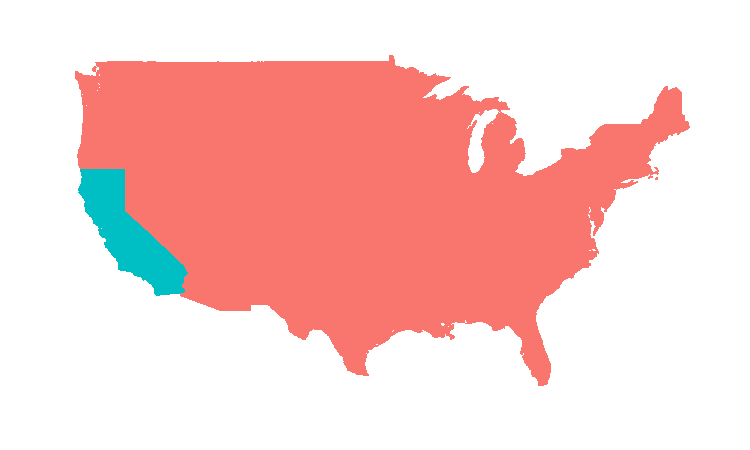
\includegraphics[width=\maxwidth]{figure/state} 

}

\caption[California Selected]{California Selected\label{fig:state}}
\end{figure}


\end{knitrout}

The hierarchy of valid geographic regions for GET requests resembles a tree structure and at the top there is a country-wide geography; this is data aggregated among all states and corresponds to summary level 010 from table \ref{tab:geolist}.  Below a country-wide summary the Census Bureau has a state-level geography.  At this level it is possible to request data for all states or for particular states; this is summary level 040.  In figure \ref{fig:state} California is selected with the following HTTP GET request: \url{http://api.census.gov/data/[YEAR]/[DATASET]?key=[KEY]&get=[VARIABLES]&for=state:06}.\\

\begin{knitrout}
\definecolor{shadecolor}{rgb}{0.969, 0.969, 0.969}\color{fgcolor}\begin{figure}[]


{\centering 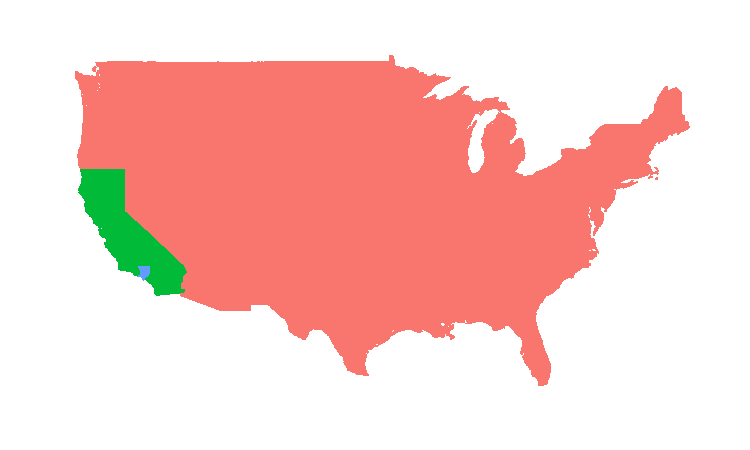
\includegraphics[width=\maxwidth]{figure/county} 

}

\caption[Los Angeles county selected]{Los Angeles county selected\label{fig:county}}
\end{figure}


\end{knitrout}

Below states there are counties and census tracts.  County level requests require specifying a containing state.  After specifying our containing state California it is possible to request county-level data (summary level 050).  From figure \ref{fig:county}, Los Angeles county within the state of California is selected.  This corresponds to an HTTP GET request of the following form: \url{http://api.census.gov/data/[YEAR]/[DATASET]?key=[KEY]&get=[VARIABLES]&for=county:037&in=state:06}.  There are a few other geographic regions avaiable within a state such as ZIP code tabulation area; for example it is possible to form a valid GET request to select ZIP code region 90210 which corresponds to Beverly Hills, California.\\
\begin{knitrout}
\definecolor{shadecolor}{rgb}{0.969, 0.969, 0.969}\color{fgcolor}\begin{figure}[]


{\centering 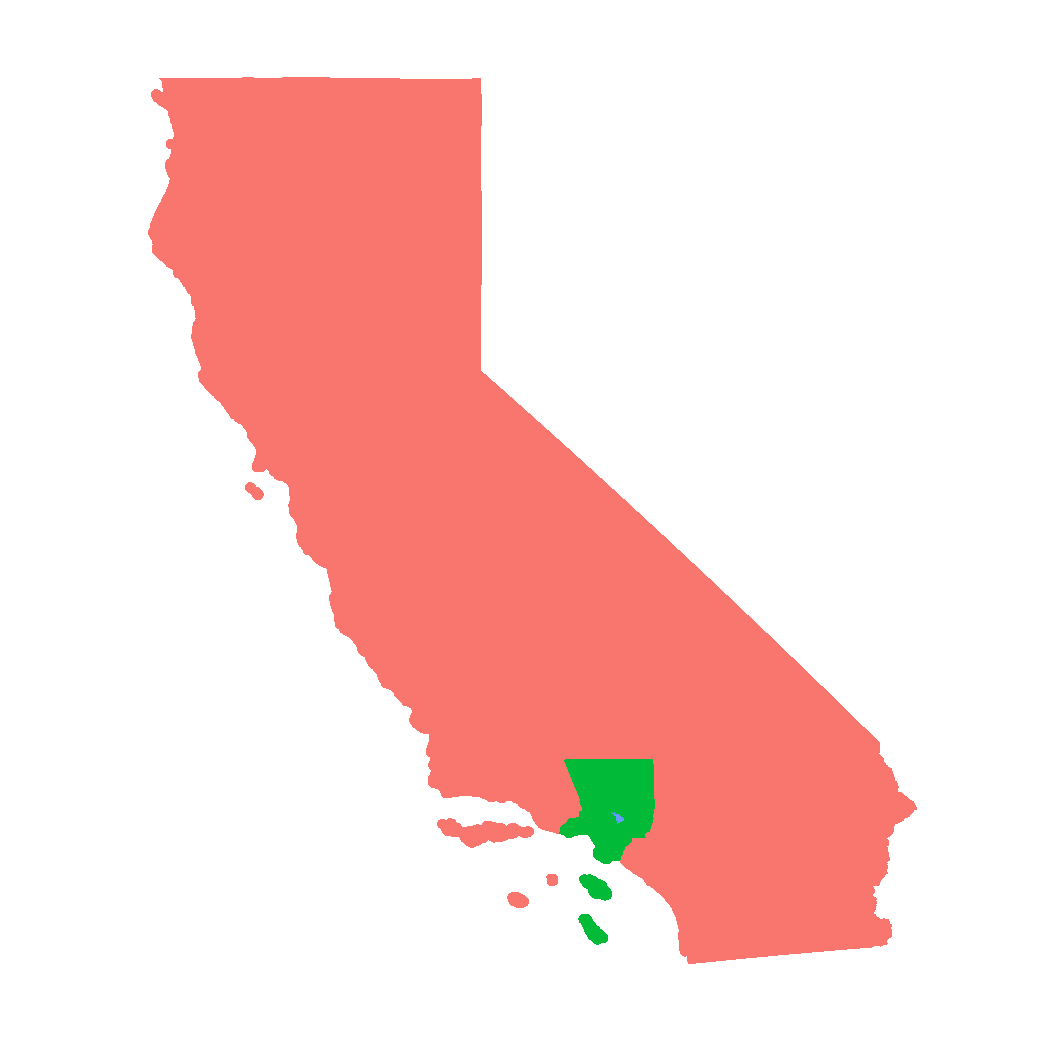
\includegraphics[width=3in]{figure/censustractstate1} 

\includegraphics[width=3in]{figure/censustractstate2} 

}

\caption[Pasadena county subdivision selected]{Pasadena county subdivision selected\label{fig:censustractstate}}
\end{figure}


\end{knitrout}

There are a number of valid geographic entities below the state and county level.  For example, there are school districts, county subdivision, metropolitan statistical areas and legislative districts.  In order to form a valid HTTP GET request, smaller geographic divisions often require specify the containing state or county.  In figure \ref{fig:censustractstate} Pasadena, a county subdivision within Los Angeles County is selected.  County subdivisions are nested within county and state, however it is not possible to specify the Pasadena county subdivision without specifying both California and Los Angeles County.  The reason for this is because the Census Bureau API does not recognize subdivision as a standalone geographic entity and state-subdivision is also not a valid geographic combination.  From table \ref{tab:geolist} state-county-subdivision is a valid summary level and this means that only after specifying California and Los Angeles County do we have access to the Pasadena county subdivision.  In this case county subdivisions are nested within states, but county subdivisions have a more immediate parent in the hierarchy: counties.\\
\\
Although all the entries in table \ref{tab:geolist} are valid geographic combinations, the summary levels do not indicate that some parts of geographic combinations may be optional.  The earlier discussion of JSON/XML formatting revealed that for census tracts certain elements in the containing geography can be omitted under certain cases.  Recall that for census tracts one option is to specify both the containing state and the county (summary level 140).  For census tracts, if the GET request is for all census tracts within a state, the specifying county is optional.  This is in contrast to county subdivisions where specifying both state and county is required with no option to leave out county.  This means that state-tract is also a valid geographic combination which is not indicated in table \ref{tab:geolist}.  It is best to refer to each datasets' JSON or XML file for geographic compatabilities.\\
\\
Due to the sheer number of different geographic entities there are geographic combinations which cannot be used together for valid HTTP GET requests.  Compatible geographies are generally nested.  Certain geographic regions will have conflicting borders with other geographic regions and smaller geographic divisions are not necessarily nested in one of the larger geographic divisions; for example, ZIP code areas are generally used by the United States Postal Service and might span different counties or census tracts.  Additionally, Legislative districts do not line up with county borders and school districts often do not line up with either legislative districts or county borders.  See figure \ref{fig:iowa} to see a comparison of different geographic entities within Iowa.\\
\\
From figure \ref{fig:iowa} state house districts and state senate districts share some common borders but some senate districts are comprised of multiple house districts.  In this case house districts are nested within senate districts.  Iowa's unified school districts are completely different from both house and senate districts and also do not line up with county borders.  This is an example of incompatible geographies; unified school districts are not nested in house, senate or counties and are incompatible with these geographic entities.\\

\begin{knitrout}
\definecolor{shadecolor}{rgb}{0.969, 0.969, 0.969}\color{fgcolor}\begin{figure}[]


{\centering 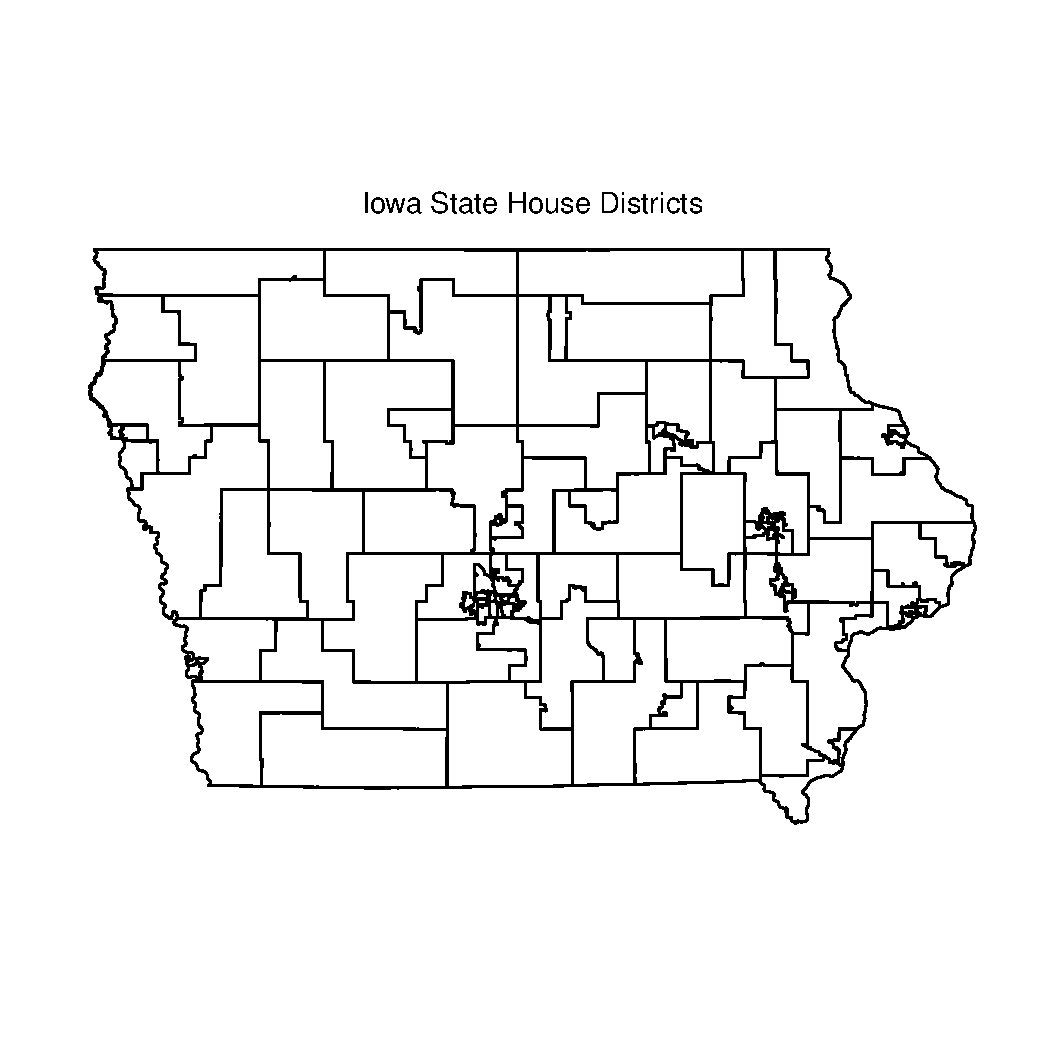
\includegraphics[width=3in]{figure/iowa1} 
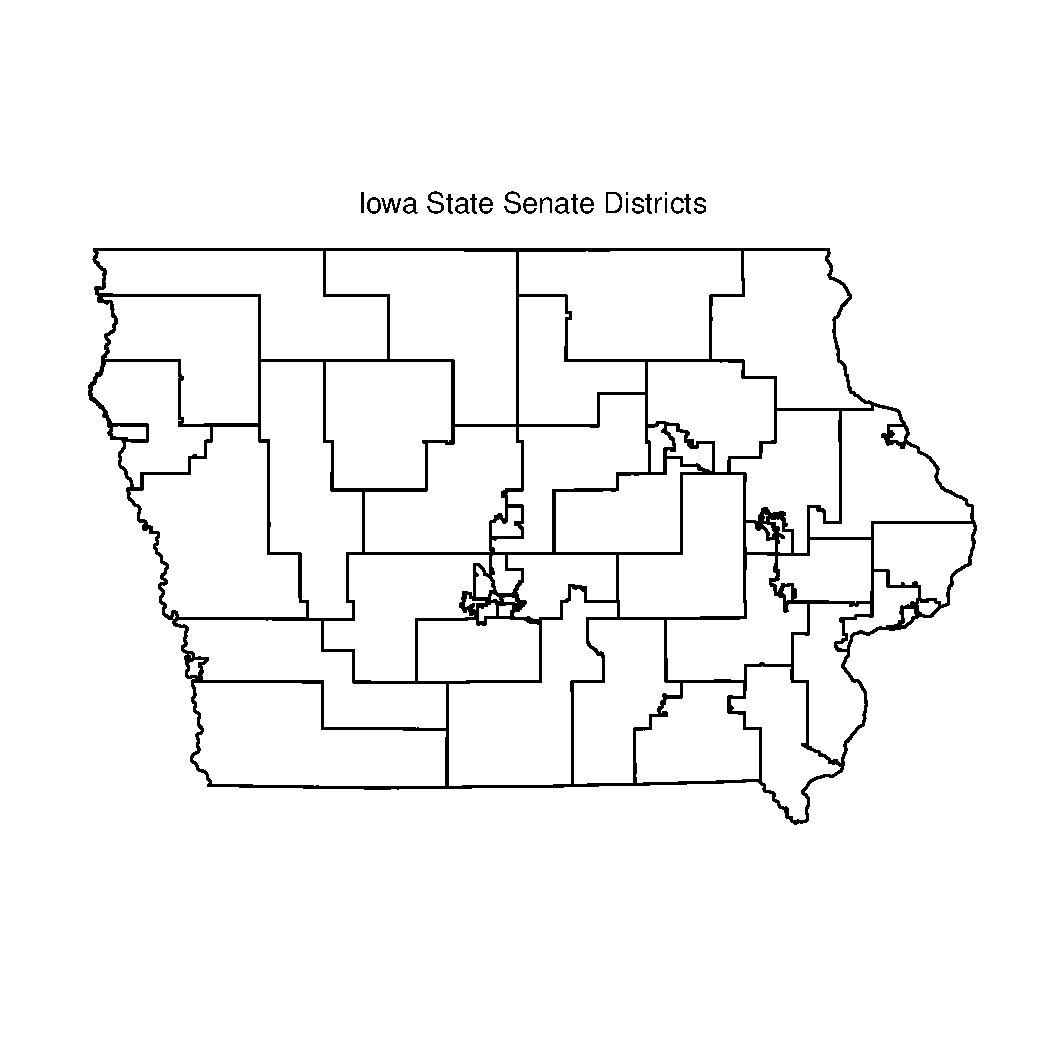
\includegraphics[width=3in]{figure/iowa2} 
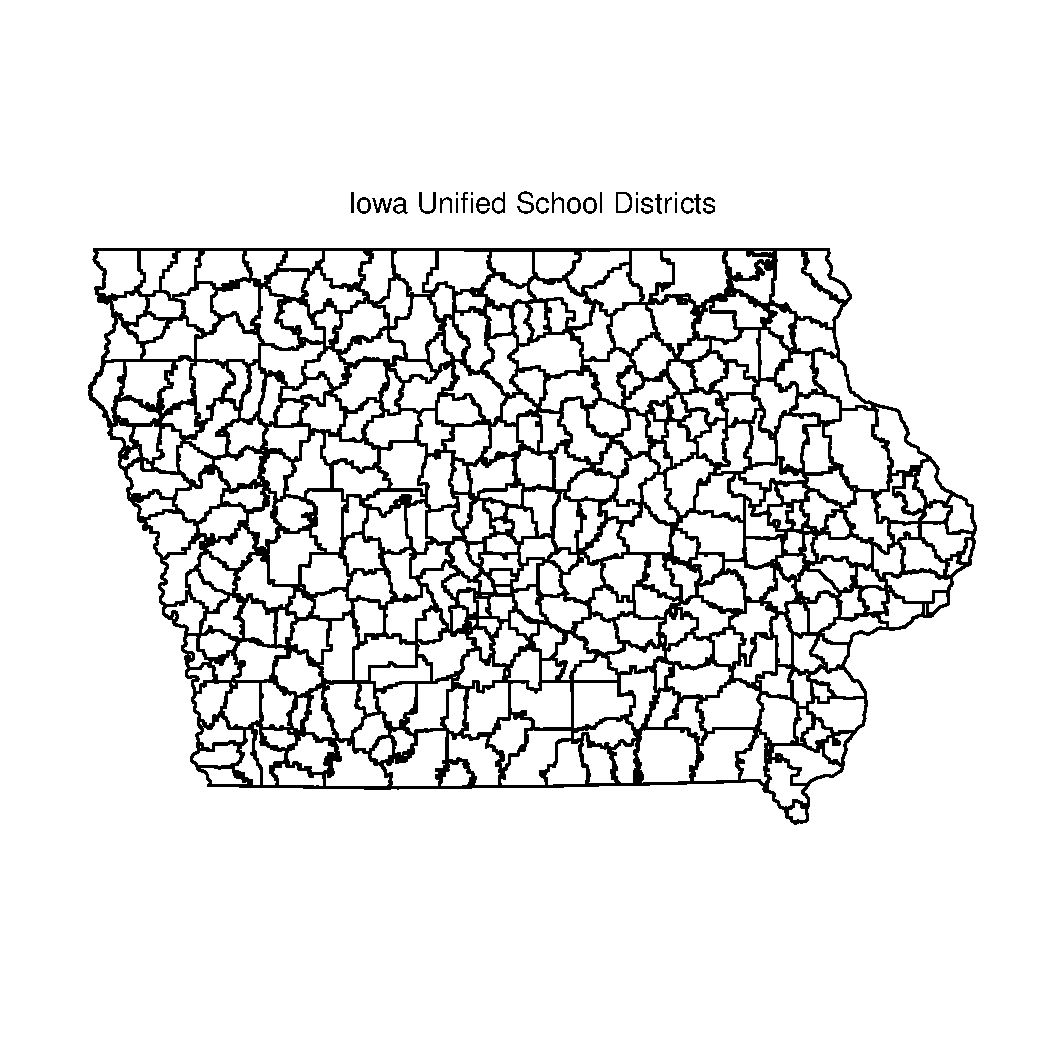
\includegraphics[width=3in]{figure/iowa3} 
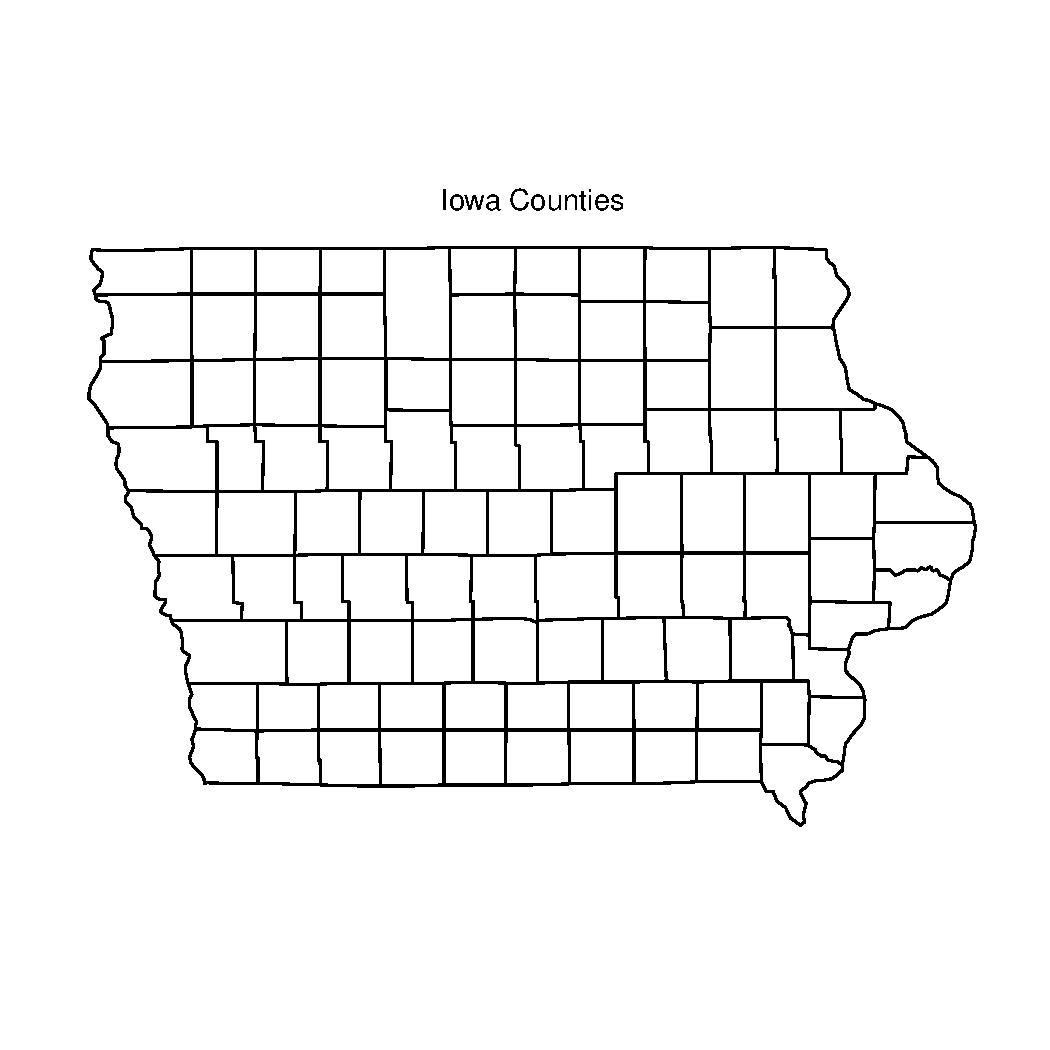
\includegraphics[width=3in]{figure/iowa4} 

}

\caption[Various geographic entities in Iowa]{Various geographic entities in Iowa\label{fig:iowa}}
\end{figure}


\end{knitrout}


For a more detailed look at which geographies need to be specified, refer to the census bureau list of summary levels for each dataset or the XML or JSON geography files.  For the 2012 ACS dataset this is located at \url{http://api.census.gov/data/2012/acs5/geo.html}, the XML file is located at \url{http://api.census.gov/data/2012/acs5/geography.xml} and the JSON file is located at \url{http://api.census.gov/data/2012/acs5/geography.json}.  The above maps are available in shapefile format from the Census Bureau website located at \url{http://www.census.gov/cgi-bin/geo/shapefiles2013/main}.

\subsection{Finding Data Sets and Tables Structure}
\label{sec:var}
The ($[$VARIABLES$]$) parameters depends on dataset.  To track which datasets are available there is a master index of available dataset formatted in both JSON and XML provided by the Census Bureau.  The JSON file is available online at \url{http://api.census.gov/data.json} and the XML file is available online at \url{http://api.census.gov/data.xml}.  This master index includes necessary meta-information about each dataset including description, links to geography and variable information and contact information for maintainer of datasets.  The JSON format is formatted as follows:
\begin{verbatim}
{
  "c_vintage": 2012,
  "c_dataset":[ 
    "acs5"
  ],
  "c_geographyLink": "http://api.census.gov/data/2012/acs5/geography.json",
  "c_variablesLink": "http://api.census.gov/data/2012/acs5/variables.json",
  "c_tagsLink": "http://api.census.gov/data/2012/acs5/tags.json",
  "c_examplesLink": "http://api.census.gov/data/2012/acs5/examples.json",
  "c_documentationLink": "http://www.census.gov/developers/",
  "c_isAggregate": true,
  "title": "2012 American Community Survey: 5-Year Estimates",
  "webService": "http://api.census.gov/data/2012/acs5",
  "accessLevel": "public",
  "bureauCode": [
    "006:07"
  ],
  "contactPoint": "Census Bureau Call Center",
  "description": "The American Community Survey (ACS) is a nationwide survey...",
  "identifier": "2012acs5",
  "mbox": "pio@census.gov",
  "publisher": "US Census Bureau",
  "references": [
    "http://www.census.gov/developers/"
  ],
  "spatial": "US",
  "temporal": "2012"
  },
}
\end{verbatim}
The above excerpt from \url{http://api.census.gov/data.json} is the meta-information about the 2008-2012 ACS 5-year dataset.  For this dataset there are links to the associated geography file and to another JSON file $variables.json$ which is a list of variables available from this dataset.  For the above example the same meta-information is formatted in XML as follows:
\begin{verbatim}
<dataset vintage="2012" 
  geographyLink="http://api.census.gov/data/2012/acs5/geography.xml"
  variablesLink="http://api.census.gov/data/2012/acs5/variables.xml" 
  tagsLink="http://api.census.gov/data/2012/acs5/tags.xml" 
  examplesLink="http://api.census.gov/data/2012/acs5/examples.xml" 
  documentationLink="http://www.census.gov/developers/" 
  pod:webService="http://api.census.gov/data/2012/acs5" isAggregate="true" 
  pod:accessLevel="public" 
  dcat:contactPoint="Census Bureau Call Center" 
  dct:identifier="2012acs5" 
  pod:mbox="pio@census.gov" 
  dct:publisher="US Census Bureau" 
  dct:spatial="US" 
  dct:temporal="2012">
<dataset-name> <part name="acs5"/> </dataset-name>
<dct:title>2012 American Community Survey: 5-Year Estimates</dct:title>
<pod:bureauCode> 006:07 </pod:bureauCode>
<dct:description>
The American Community Survey (ACS) is a nationwide survey...
</dct:description>
<pod:reference link="http://www.census.gov/developers/"/>
</dataset>
\end{verbatim}
After selecting a dataset listed in the master index, the user will lookup what variables are available for that dataset.  The JSON and XML master index of datasets contain the location of $variables.json$ and $variables.xml$ respectively which list available variables available for that dataset.  Available variables are organized into tables referred to as $concepts$; a $concept$ is a combination of factors.  For example, ``Health Insurance Coverage Status by Sex by Age" is a concept from the 2012 ACS.  Within each $concept$ are $labels$; a $label$ is a combination of levels for the factors within a concept.\\
\\
Within each concept there are multiple labels that provide information on different levels of each of the factors.  For example, the concept ``Health Insurance Coverage Status by Sex by Age" contains a label for males over 70 with health insurance.  This concept also contains labels for each combination of gender (male, female), age group (under 6, 6 to 17, 18 to 24, 25 to 34, 35 to 44, 45 to 54, 55 to 64, 65 to 74 and 75 and over) and health insurance coverage (with and without health insurance).  Some of the labels may also contain summary information in the form of totals.  For this concept there are labels for total number of males, total number of females and totals for males/females in each age group.\\
\\
To lookup what variables are available, the {\tt variables.json} and {\tt variables.xml} files contain a list of all concepts and labels along with a description.  The JSON formatted $variables.json$ is formatted as follows:
\begin{verbatim}
"B27001_056E": {
  "label": "Female:!!75 years and over:!!With health insurance coverage",
  "concept": "B27001.  Health Insurance Coverage Status by Sex by Age"
},
\end{verbatim}
This describes label 056E of concept B27001.  This is a table of 75 and older females with health insurance.  The associated XML formatted version is formatted as follows:
\begin{verbatim}
<var xml:id="B27001_056E" 
  label="Female:!!75 years and over:!!With health insurance coverage" 
  concept="B27001. Health Insurance Coverage Status by Sex by Age"/>
\end{verbatim}
In both the XML and JSON formats the different levels of factors in the labels are separated by !!.  To form a valid GET request we take the header from the JSON file (or the $id$ from the XML file) and that will be the parameter we use for ($[$VARIABLES$]$).  The concept-label ID $B27001\_056E$ will request the ``75 and older female with health insurance" label from the ``health insurance coverage status by sex by age" concept.  A valid HTTP GET request for this is \url{http://api.census.gov/data/[YEAR]/[DATASET]?key=[KEY]&get=B27001_056E&for=[GEOGRAPHY]}.

% latex table generated in R 3.0.2 by xtable 1.7-3 package
% Mon Apr 14 22:35:14 2014
\begin{table}[ht]
\centering
\begin{tabular}{rlllll}
  \hline
 & B27001\_056E & B27001\_056E & NAME & state & county \\ 
  \hline
2 & 45052 & 45052 & Alameda County, California & 06 & 001 \\ 
  3 & 18 & 18 & Alpine County, California & 06 & 003 \\ 
  4 & 1733 & 1733 & Amador County, California & 06 & 005 \\ 
  5 & 9431 & 9431 & Butte County, California & 06 & 007 \\ 
  6 & 1938 & 1938 & Calaveras County, California & 06 & 009 \\ 
  7 & 582 & 582 & Colusa County, California & 06 & 011 \\ 
   \hline
\end{tabular}
\caption{Health insurance status of women 75 years and older in California by county from 2012 ACS 5-year data} 
\label{tab:df}
\end{table}



Table \ref{tab:df} is information on health insurance for women 75 and older in California from the 2012 ACS 5-year data listed by county.  The HTTP GET request for this is \url{http://api.census.gov/data/2012/acs5?key=[KEY]&get=B27001_056E,B27001_057E,NAME&for=county:*&in=state:06}.  Labels 056E and 057E are labels for women 75 and older with health insurance and women 75 and older without health insurance respectively.  The result of our HTTP GET request is a JSON formatted file in the following format:
\begin{verbatim}
[["B27001_056E","B27001_057E","NAME","state","county"],
["668","144","Alameda County, California","06","001"],
["15","69","Alpine County, California","06","003"],
["88","131","Amador County, California","06","005"],
["238","127","Butte County, California","06","007"],
["45","102","Calaveras County, California","06","009"],
["98","26","Colusa County, California","06","011"],
\end{verbatim}
This indicates that there are 668 women over 75 in Alameda county that have health insurance and 144 women over 75 in Alameda county without health insurance.\\
\\
The list of variables, $variables.json$ and $variables.xml$ not only contain a list of variables as described above but also include margin of error.  Estimates from the ACS are based on random sampling thus each of the estimates has a standard error.  The Census Bureau uses a 90$\%$ confidence level for their margin of error.  To find the associated margin of error for our variable we replace the last letter of label with an ``M" instead of an ``E".  For example, $B27001\_056E$ and $B27001\_057E$ are the associated standard errors for the previous example.  Standard errors have the exact same formatting as any other variable from the ACS:
\begin{verbatim}
[["B27001_056M","B27001_057E","NAME","state","county"],
["356","302","Alameda County, California","06","001"],
["13","0","Alpine County, California","06","003"],
["51","0","Amador County, California","06","005"],
["134","47","Butte County, California","06","007"],
["99","0","Calaveras County, California","06","009"],
["34","0","Colusa County, California","06","011"],
\end{verbatim}
Using the above table, $668 \pm 356$ is a 90$\%$ confidence interval for the number of women in Alameda County 75 and over with health insurance.

\section{Limitations of the API}
\citet{stangl:2013} talks about using the ACS as a dataset for classroom exercises because it demonstrates how statistics are used to make important policy decisions.  This article contains a number of classroom exercises that ask the reader to calculate some basic proportions about various demographic data such as health insurance coverage, marriage status and income.  The particular dataset used by \citet{stangl:2013} is a 1000 observation random subset of the 2010 ACS public use microdata sample.  We will attempt to use the Census Bureau online API to examine the same demographic variables.\\
\\
Using the Census Bureau's online API for these exercises presents us three main problems.  
\begin{enumerate}
\item The structure of data in the public use microdata sample is different from data from the online API.
\item Proportions and standard errors are not included.
\item Certain combination of variables are simply not available from the online API.
\end{enumerate}

% latex table generated in R 3.0.2 by xtable 1.7-3 package
% Mon Apr 14 20:37:10 2014
\begin{table}[ht]
\centering
\begin{tabular}{rrrrrlrrr}
  \hline
Sex & Age & Married & Income & HoursWk & Race & USCitizen & HealthInsurance & Language \\ 
  \hline
  0 &  31 &   0 & 60.00 &  40 & white &   1 &   1 &   1 \\ 
    1 &  31 &   0 & 0.36 &  12 & black &   1 &   1 &   0 \\ 
    1 &  75 &   0 & 0.00 &  & white &   1 &   1 &   0 \\ 
    0 &  80 &   0 & 0.00 &  & white &   1 &   1 &   0 \\ 
    1 &  64 &   1 & 0.00 &  & white &   1 &   1 &   0 \\ 
    1 &  14 &   0 &  &  & white &   1 &   1 &   0 \\ 
   \hline
\end{tabular}
\caption{Random subset of 2010 ACS public use microdata sample} 
\label{tab:table}
\end{table}


Data from the ACS public use microdata sample is organized to describe individuals.  Each row of the dataset describes an anonymized individual and each column represents a different demographic variable.  See table \ref{tab:table} for a small subset of the data used by Morgan et al.\\
% latex table generated in R 3.0.2 by xtable 1.7-1 package
% Tue Mar 25 23:20:04 2014
\begin{table}[ht]
\centering
\begin{tabular}{rrrrrr}
  \hline
 & Total & M Total & M $<$6 & M $<$6 w/insurance & M $<$6 w/o insurance \\ 
  \hline
Alabama & 4693822 & 2256713 & 186155 & 176591 & 9564 \\ 
  Alaska & 686905 & 349855 & 33053 & 29026 & 4027 \\ 
  Arizona & 6304406 & 3099407 & 279297 & 249163 & 30134 \\ 
  Arkansas & 2862023 & 1394466 & 120828 & 115053 & 5775 \\ 
  California & 36783532 & 18138870 & 1561623 & 1461559 & 100064 \\ 
  Colorado & 4949633 & 2457605 & 210948 & 193227 & 17721 \\ 
   \hline
\end{tabular}
\caption{Health Insurance Coverage information from Census API.  Each of the M columns indicate male, subsequent numbers indicate age; there are corresponding F columns for females that is not shown to conserve space.} 
\label{fig:example}
\end{table}


By contrast the online API does not provide individual specific data.  When we perform a HTTP GET request we must specify what geographic level of detail we want.  The geographic level of detail does not go below the county subdivision or census tract level.  Instead of individual specific data we have data that has been aggregated for an entire geographic region.  This is likely due to privacy reasons; if we have individual specific data for a dozen demographic variables along with geographic information it might be possible to reveal this individual's identity.  \\
\\
In table \ref{fig:example} we specify state level summaries for health insurance coverage status for various age groups by gender (from the census API this is table B27001).  Each variable is in the form of a table and as previously mentioned we refer to this as a $concept$ and each column in table \ref{fig:example} is referred a $label$.  The first label of each concept is an overall total; the total number of people in the specified geographic region that answered questions relating to the requested concept.   Subsequent labels are subsets of this overall total.  We've conveniently renamed column headers in table \ref{fig:example}; the naming convention from data provided by the API is to enumerate each label with the table name: $B27001\_001$, $B27001\_002$ etc.\\
\\
The way this data is organized is not tidy $<$include hadley tidy data reference$>$.  Instead it appears that the columns contain additional categorical information: gender, age and insurance.  In table \ref{fig:tidy} we have tidied up the data so that each row is an observation and each column is a variable.  Originally table B27001 contains a number of $total$ columns: overall total, total number of males, total number of females, and within each gender a total number of people within an age group.  In reshaping this data, we felt that these total columns were redundant once the data is in a tidy form. \\

% latex table generated in R 3.0.2 by xtable 1.7-3 package
% Mon Apr 14 20:37:10 2014
\begin{table}[ht]
\centering
\begin{tabular}{llllr}
  \hline
state & gender & age & insurance & freq \\ 
  \hline
Alabama & m & $<$6 & yes & 176591 \\ 
  Alaska & m & $<$6 & yes & 29026 \\ 
  Arizona & m & $<$6 & yes & 249163 \\ 
  Arkansas & m & $<$6 & yes & 115053 \\ 
  California & m & $<$6 & yes & 1461559 \\ 
  Colorado & m & $<$6 & yes & 193227 \\ 
   \hline
\end{tabular}
\caption{Reshaped Health Insurance Coverage data.} 
\label{fig:tidy}
\end{table}



The Census Bureau has historically provided information in the form of a count.  However, the nominal frequency of variables may not hold much meaning as different geographic entities contain different populations.  For example, in table \ref{tab:freq} we have university enrollment by age and gender for each state from the 2012 5-year ACS dataset.  This dataset is reshaped into a tidy form.  In this dataset we have gender, age and enrollment status (public university, private university or not enrolled).  California had over 700,000 male students at public universities while Colorado only had around 80,000 students in the same category.  These nominal enrollment numbers mean very little without knowing the size of the population.\\
% latex table generated in R 3.0.2 by xtable 1.7-3 package
% Mon Apr 14 21:27:16 2014
\begin{table}[ht]
\centering
\begin{tabular}{llllr}
  \hline
state & gender & school & age & freq \\ 
  \hline
Alabama & m & public & 18.to.24 & 73085 \\ 
  Alaska & m & public & 18.to.24 & 7852 \\ 
  Arizona & m & public & 18.to.24 & 98686 \\ 
  Arkansas & m & public & 18.to.24 & 41490 \\ 
  California & m & public & 18.to.24 & 713506 \\ 
  Colorado & m & public & 18.to.24 & 84460 \\ 
   \hline
\end{tabular}
\caption{University enrollment by gender, age and university type} 
\label{tab:freq}
\end{table}


The size of the population depends on the topic of interest.  One potential topic of interest is gender differences in public university enrollment in college aged individuals.  In this case our population is the total number of college aged students enrolled in a public university.  In table \ref{tab:freq2}, we modify the above table and calculate the percentage of males/females for each combination of school and age group for each state.\\
% latex table generated in R 3.0.2 by xtable 1.7-3 package
% Mon Apr 14 23:38:48 2014
\begin{table}[ht]
\centering
\begin{tabular}{llllr}
  \hline
state & gender & school & age & pct \\ 
  \hline
Alabama & m & public & 18.to.24 & 0.44 \\ 
  Alaska & m & public & 18.to.24 & 0.45 \\ 
  Arizona & m & public & 18.to.24 & 0.46 \\ 
  Arkansas & m & public & 18.to.24 & 0.46 \\ 
  California & m & public & 18.to.24 & 0.48 \\ 
  Colorado & m & public & 18.to.24 & 0.49 \\ 
   \hline
\end{tabular}
\caption{University enrollment by gender, age and university type} 
\label{tab:freq2}
\end{table}


These percentages tell us a lot more about the data; when it comes to public university enrollment for college-aged invidividuals both California and Colorado have fewer males enrolled.  Finding these proportions was not difficult but it requires a bit more work to correctly add up the frequencies in our population.\\
\\
A more difficult problem is in finding standard errors for confidence intervals.  Recall that the Census Bureau provides a margin of error for each variable at the 90$\%$ confidence level.  Finding standard errors (SE) for the estimates from the margin of error (MOE) is straight forward: $SE = \frac{MOE}{1.645}$ where 1.645 is the critical value from the standard normal distribution that corresponds to a central area of $0.90$.  Finding the standard error for proportions requires further calculations:
\begin{align*}
SE(\frac{A}{B}) = \frac{1}{B}\sqrt{SE(A)^2 - (\frac{A}{B})^2 SE(B)^2}
\end{align*}
In calculating proportions we must often add different estimates together for different $labels$.  Combining the standard error for a sum of estimates: $SE(A + B) = \sqrt{SE(A)^2 + SE(B)^2}$.\\
%https://www.census.gov/acs/www/Downloads/data_documentation/Statistical_Testing/2012StatisticalTesting3and5.pdf
\\
Due to how the data is provided by the Census Bureau compared with the subset of the public use microsample that is used in \citet{stangl:2013} there are limited combination of variables that are available.  One of the exercises in \citet{stangl:2013} is to compare health insurance status by race.  This exercise using the public use microsample is straight forward and requires a single line of code using the plyr package in R.  We can summarise percentage of people with health insurance by race as follows:
\begin{knitrout}
\definecolor{shadecolor}{rgb}{0.969, 0.969, 0.969}\color{fgcolor}\begin{kframe}
\begin{alltt}
\hlkwd{library}\hlstd{(plyr)}
\hlstd{acsdat} \hlkwb{=} \hlkwd{read.csv}\hlstd{(}\hlstr{"datasetSTANGL2013.csv"}\hlstd{)}  \hlcom{#Stangl's dataset}
\hlkwd{head}\hlstd{(acsdat)}
\end{alltt}
\begin{verbatim}
##   Sex Age Married Income HoursWk  Race USCitizen HealthInsurance Language
## 1   0  31       0  60.00      40 white         1               1        1
## 2   1  31       0   0.36      12 black         1               1        0
## 3   1  75       0   0.00      NA white         1               1        0
## 4   0  80       0   0.00      NA white         1               1        0
## 5   1  64       1   0.00      NA white         1               1        0
## 6   1  14       0     NA      NA white         1               1        0
\end{verbatim}
\begin{alltt}
\hlstd{acsdat_by_race} \hlkwb{=} \hlkwd{ddply}\hlstd{(acsdat,} \hlkwd{.}\hlstd{(Race), summarise,} \hlkwc{insurance_pct} \hlstd{=} \hlkwd{sum}\hlstd{(HealthInsurance)}\hlopt{/}\hlkwd{length}\hlstd{(Race))}
\hlkwd{print}\hlstd{(acsdat_by_race)}
\end{alltt}
\begin{verbatim}
##    Race insurance_pct
## 1 asian        0.8429
## 2 black        0.8113
## 3 other        0.7302
## 4 white        0.8804
\end{verbatim}
\end{kframe}
\end{knitrout}

This same calculation can be done from data provided by the online API.  Recall that the data at the individual data is not available with the online API but it is still to calculate overall insurance rates using state or country level data.  An additional step is required because the online API separates race into eight separate tables.  Due to the structure of the data from the ACS package, without putting the data in tidy form, finding the percentage with health insurance requires summing columns and element-wise division between columns.  


\begin{knitrout}
\definecolor{shadecolor}{rgb}{0.969, 0.969, 0.969}\color{fgcolor}\begin{kframe}
\begin{alltt}
\hlcom{# column names from ACS}
\hlkwd{print}\hlstd{(}\hlkwd{colnames}\hlstd{(health_white))}
\end{alltt}
\begin{verbatim}
##  [1] "Health Insurance Coverage Status by Age (White Alone): Total:"                                           
##  [2] "Health Insurance Coverage Status by Age (White Alone): Under 18 years:"                                  
##  [3] "Health Insurance Coverage Status by Age (White Alone): Under 18 years: With health insurance coverage"   
##  [4] "Health Insurance Coverage Status by Age (White Alone): Under 18 years: No health insurance coverage"     
##  [5] "Health Insurance Coverage Status by Age (White Alone): 18 to 64 years:"                                  
##  [6] "Health Insurance Coverage Status by Age (White Alone): 18 to 64 years: With health insurance coverage"   
##  [7] "Health Insurance Coverage Status by Age (White Alone): 18 to 64 years: No health insurance coverage"     
##  [8] "Health Insurance Coverage Status by Age (White Alone): 65 years and over:"                               
##  [9] "Health Insurance Coverage Status by Age (White Alone): 65 years and over: With health insurance coverage"
## [10] "Health Insurance Coverage Status by Age (White Alone): 65 years and over: No health insurance coverage"
\end{verbatim}
\begin{alltt}
\hlcom{# sums columns together}
\hlstd{calc_pct} \hlkwb{=} \hlkwa{function}\hlstd{(}\hlkwc{df}\hlstd{) \{}
    \hlkwd{sum}\hlstd{(df[}\hlkwd{c}\hlstd{(}\hlnum{3}\hlstd{,} \hlnum{6}\hlstd{,} \hlnum{9}\hlstd{)])}\hlopt{/}\hlstd{df[,} \hlnum{1}\hlstd{]}
\hlstd{\}}

\hlcom{# sum columns}
\hlstd{a_pct} \hlkwb{=} \hlkwd{calc_pct}\hlstd{(health_asian)}
\hlstd{b_pct} \hlkwb{=} \hlkwd{calc_pct}\hlstd{(health_black)}
\hlstd{o_pct} \hlkwb{=} \hlkwd{calc_pct}\hlstd{(health_other)}
\hlstd{w_pct} \hlkwb{=} \hlkwd{calc_pct}\hlstd{(health_white)}
\end{alltt}
\end{kframe}
\end{knitrout}

The column headers of the health insurance by race dataset from the online API reveal one big issue: the available variables are strictly set and cannot be easily changed.  The original exercise was to calculate health insurance coverage percentage for each race and age group is not a variable of interest.  In the subset of the public use microsample in \citet{stangl:2013} there were additional variables but because this dataset is in a tidy format it is possible to easily subset the data by row.  The dataset from the online API has different levels of factors in each column, age and health insurance status, and requires an extra step to sum health insurance numbers over the different levels of the age variable.  For datasets with more variables than just age and health insurance coverage, the non-tidy structure of this data means that summaries of some of the variables will requiring summing over all levels of other variables.  For each of the different datasets for races we have summed up health insurance coverage numbers over the different age groups and found the overall health coverage percentage numbers:
\begin{knitrout}
\definecolor{shadecolor}{rgb}{0.969, 0.969, 0.969}\color{fgcolor}\begin{kframe}
\begin{verbatim}
## [1] "asian insurance_pct: 0.851522"
## [1] "black insurance_pct: 0.825249"
## [1] "other insurance_pct: 0.733575"
## [1] "white insurance_pct: 0.868986"
\end{verbatim}
\end{kframe}
\end{knitrout}

Since the available variables are strictly set, it is not possible to subset further.  From the dataset in \citet{stangl:2013}, it is possible to subset further: health insurance percentage by race and gender.  Again, this calculation requires one line of code using the plyr package in R:
\begin{knitrout}
\definecolor{shadecolor}{rgb}{0.969, 0.969, 0.969}\color{fgcolor}\begin{kframe}
\begin{alltt}
\hlkwd{library}\hlstd{(plyr)}
\hlstd{acsdat} \hlkwb{=} \hlkwd{read.csv}\hlstd{(}\hlstr{"datasetSTANGL2013.csv"}\hlstd{)}  \hlcom{#Stangl's dataset}
\hlkwd{head}\hlstd{(acsdat)}
\end{alltt}
\begin{verbatim}
##   Sex Age Married Income HoursWk  Race USCitizen HealthInsurance Language
## 1   0  31       0  60.00      40 white         1               1        1
## 2   1  31       0   0.36      12 black         1               1        0
## 3   1  75       0   0.00      NA white         1               1        0
## 4   0  80       0   0.00      NA white         1               1        0
## 5   1  64       1   0.00      NA white         1               1        0
## 6   1  14       0     NA      NA white         1               1        0
\end{verbatim}
\begin{alltt}
\hlstd{acsdat_gender_race} \hlkwb{=} \hlkwd{ddply}\hlstd{(acsdat,} \hlkwd{.}\hlstd{(Race, Sex), summarise,} \hlkwc{insurance_pct} \hlstd{=} \hlkwd{sum}\hlstd{(HealthInsurance)}\hlopt{/}\hlkwd{length}\hlstd{(Race))}
\hlkwd{print}\hlstd{(acsdat_gender_race)}
\end{alltt}
\begin{verbatim}
##    Race Sex insurance_pct
## 1 asian   0        0.9333
## 2 asian   1        0.7750
## 3 black   0        0.8833
## 4 black   1        0.7174
## 5 other   0        0.7273
## 6 other   1        0.7333
## 7 white   0        0.8720
## 8 white   1        0.8905
\end{verbatim}
\end{kframe}
\end{knitrout}

The dataset from the online API for health insurance by age and race does not include gender and because the available variables are strictly set for each table it is not possible to calculate health insurance coverage percentage by race and gender.  Our only option is to look at other tables and find one that includes all combinations of variables of interest.  There is another table available from the online API for health insurance: table number $B27001$.  This table is health insurance coverage status by age and gender.  It is possible to use both of these tables on health insurance to calculate estimates of health insurance coverage by gender and race but constructing exact figures is not possible.\\
\\



\section{Other Issues}
%\subsection{Comparing across years}
%http://www.census.gov/acs/www/guidance_for_data_users/comparing_data/
Although the ACS is a yearly survey, in its current form it is difficult to compare variables across years.  The online API has ACS data available for 2010 to 2012 but even for these years it is difficult track changes during these years.  Recall that the 2012 ACS 5-year dataset is data aggregated from 2008 - 2012.  This means that the 2010, 2011 and 2012 ACS 5-year datasets will include overlapping time periods; some of the data used aggregated to form these 5-year estimates will overlap.  \\
\\
It is possible to circumvent this overlapping data problem by combining the ACS 5-year estimate with the ACS 1-year estimate.  The 2011 ACS 5-year and the 2012 ACS 1-year do not contain overlapping data.  However, datasets from different years contain different demographic variables.  For example, questions regarding healthcare were first added in 2008 and datasets prior to 2008 will not contain healthcare variables.  The ACS 1-year estimates have smaller sample sizes and as a result not all geographic regions are available.  The ACS 1-year estimates only have data available for geographic regions with populations of 65,000 or greater.\\
\\
As a guideline the Census Bureau recommends comparing similar length datasets that do not overlap.  For example, comparing 1-year estimates from different years or 3-year estimates for two periods that don't overlap.  Unfortunately, the only option for comparing data across years out of the available datasets from the online API is to compare 2011 and 2012 1-year estimates.
%\subsection{Nonresponse}


\section{Examples from ACS}
\begin{knitrout}
\definecolor{shadecolor}{rgb}{0.969, 0.969, 0.969}\color{fgcolor}
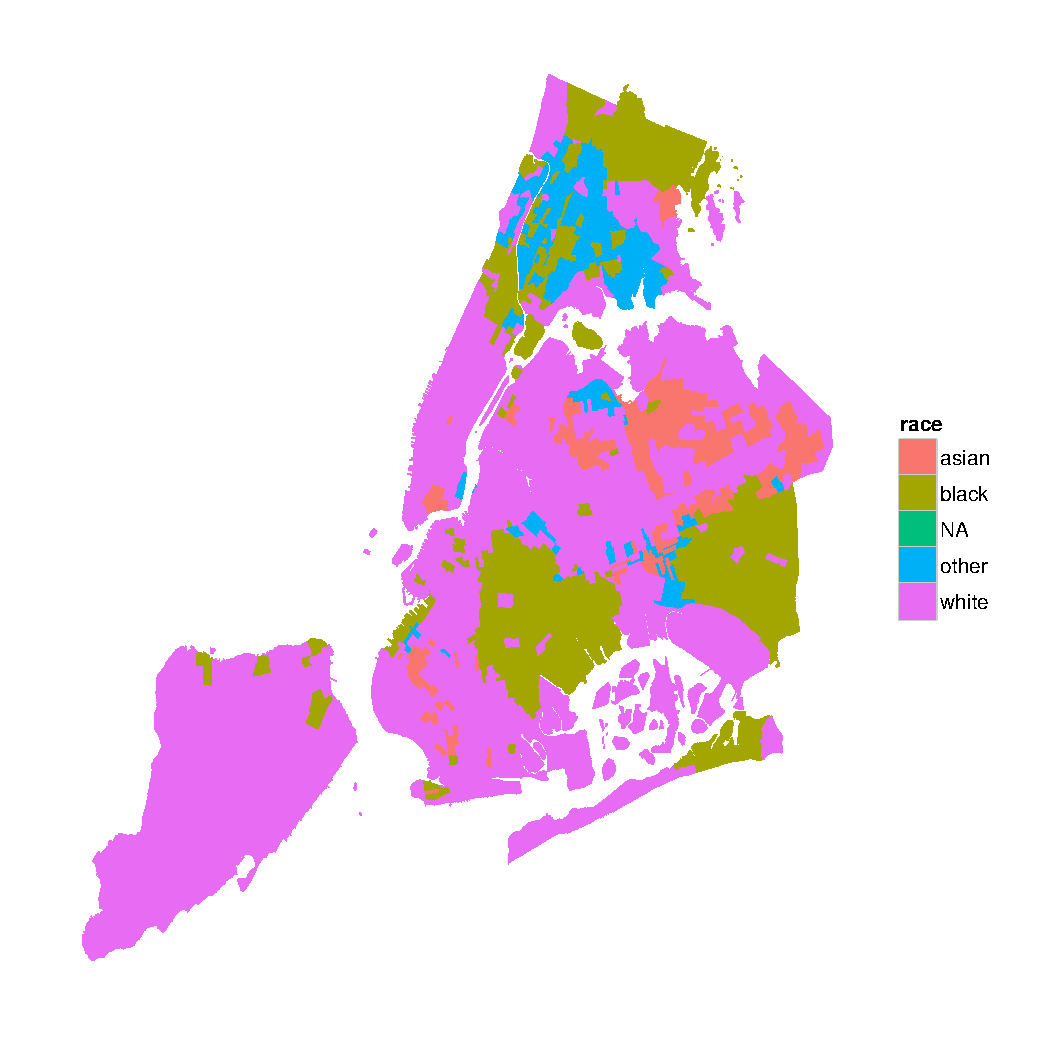
\includegraphics[width=\maxwidth]{figure/NY} 

\end{knitrout}


\begin{knitrout}
\definecolor{shadecolor}{rgb}{0.969, 0.969, 0.969}\color{fgcolor}
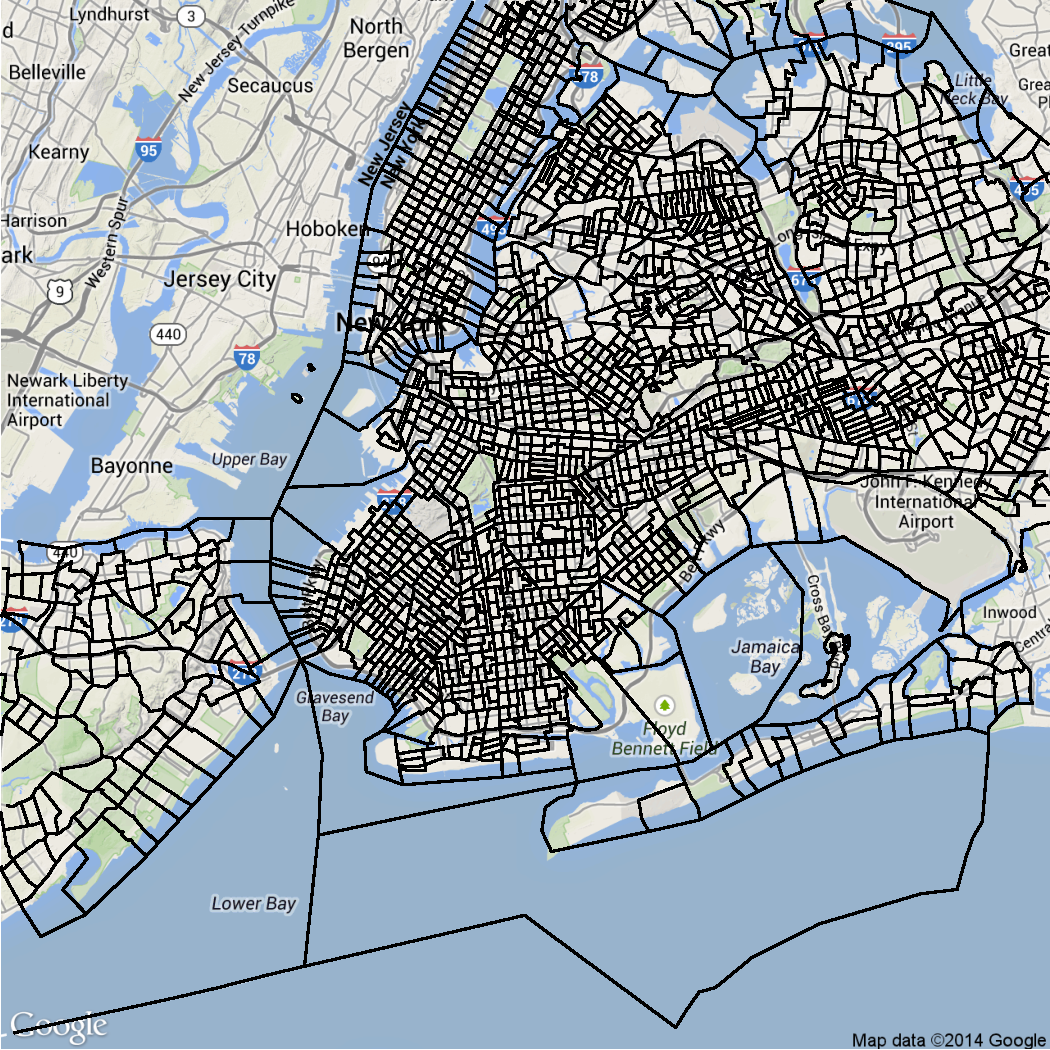
\includegraphics[width=\maxwidth]{figure/test} 

\end{knitrout}

\section{Conclusion}
The Census Bureau has created numerous tools to make it easier for the public to access their data.  These tools include Easy Stats (\url{http://www.census.gov/easystats/}), QuickFacts (\url{http://quickfacts.census.gov/qfd/index.html}), DataFerrett (\url{http://dataferrett.census.gov/}), FTP access to data tables and summary files (\url{http://www2.census.gov/}), the online developer's API (\url{api.census.gov}) and numerous other tools.  Each of these tools is targetted for a different audience: congressional staffers, emergency planners, business owners or others who need access to demographic data.  Who is the target audience for the online developer's API?\\
\\
Due to the technical knowledge required to access the online API, clearly the audience is not local business leaders or congressional staffers.  It is unlikely someone without significant programming knowledge would be able to understand the JSON and XML formats required to find datasets and variables.  Due to the structure of the data and the emphasis on frequency instead of proportions, the online API is also not designed for statisticians.  The form of the data limits the available variables for each data table and makes it difficult to subset on variables.  Right now the online API is only useful to application developers who cannot store the contents of the entire ACS datasets.  With some restructuring the API could be a useful tool for statisticians since it allows for a detailed look down to the census tract level and it allows access to data without downloading the entire dataset.

\section{Appendix}

\printbibliography

\end{document}
